% Comprehensive, expanded report for CA5 Q1 — Intelligent Law-Document Retrieval System
\documentclass[12pt,a4paper]{article}
\usepackage[margin=1in]{geometry}
\usepackage{graphicx}
\usepackage{float}
\usepackage{booktabs}
\usepackage{hyperref}
\usepackage{parskip}
\usepackage{caption}
\usepackage{tikz}
\usepackage{pgfplots}
\pgfplotsset{compat=1.17}
\usepackage{listings}
\usepackage{amsmath}
\usepackage{amssymb}
\usepackage{longtable}
\usepackage{multirow}
\usepackage{enumitem}
\usepackage{xcolor}
\usepackage{tcolorbox}
\usepackage{csquotes}
\usepackage{appendix}
\usepackage{verbatim}

\definecolor{codegray}{gray}{0.95}
\lstset{backgroundcolor=\color{codegray},basicstyle=\ttfamily\small,breaklines=true,frame=single}

\title{Report — Intelligent Law-Document Retrieval System (Assignment CA5 Q1)}
\author{Student: \\ \texttt{YOUR\_NAME} \\ Student ID: \texttt{YOUR\_ID}}
\date{\today}

\begin{document}
\maketitle
\begin{abstract}
This document presents an in-depth description of an intelligent retrieval system built to answer Persian legal questions over a local document corpus. The implementation (delivered as a Jupyter Notebook and supporting Python modules) implements a modular retrieval-augmented pipeline including: dataset preparation and cleaning, TF-IDF indexing (reference implementation), query rewriting, rule-based intent classification, metadata extraction, context retrieval with metadata filtering, reranking, and conservative extractive answer aggregation. The report explains underlying concepts, provides mathematical and algorithmic details, gives concrete implementation choices and parameters, shows sample experimental results, and provides reproducibility instructions and suggested extensions for production-grade deployment.
\end{abstract}

\tableofcontents
\clearpage

\section{Introduction}
\subsection{Motivation}
Access to legal knowledge is essential for both citizens and practitioners. Documents are long, structured, and often written in formal language where simple keyword search may miss paraphrased or context-dependent answers. RAG-style systems combine retrieval (find relevant evidence) and generation (synthesize concise answers) to produce grounded outputs with citations — a useful model for legal retrieval.

\subsection{Scope and assumptions}
This project focuses on building a reproducible, explainable pipeline that can run locally without cloud services. We assume access to plain text or OCR'ed documents and emphasize conservative, extractive approaches to minimize hallucination risks.

\subsection{Contributions}
The deliverables include:
\begin{itemize}
  \item A documented notebook implementing the pipeline and experiments.
  \item A TF-IDF based vector index and an interface for retrieval and filtering.
  \item Basic evaluation scripts computing relevancy, faithfulness, and Hit@k metrics.
  \item A Chainlit-based minimal UI for interactive exploration, and a LaTeX report (this file).
\end{itemize}

\subsubsection{Key Innovations}
\begin{itemize}
  \item Modular pipeline for easy extension to dense embeddings or LLMs.
  \item Rule-based components for interpretability and low resource usage.
  \item Metadata filtering to handle legal specificity (e.g., year-based queries).
  \item Conservative extractive generation to ensure fidelity and reduce hallucinations.
\end{itemize}

\subsubsection{Deliverables Breakdown}
\begin{itemize}
  \item \texttt{NLP\_HW5\_Q1.ipynb}: Core implementation with data loading, indexing, pipeline functions, timing, evaluation, and UI code.
  \item \texttt{app.py}: Interactive Chainlit app for user queries.
  \item \texttt{build\_submission.py}: Script to package artifacts into a ZIP.
  \item Data files: Indexed dataset, timings CSV, evaluation Excel.
  \item This report: Comprehensive LaTeX document with concepts, code, results, and appendices.
\end{itemize}

\subsection{System Architecture Overview}
The system is designed as a modular RAG pipeline: Input query → Query Rewriting → Intent Classification → Metadata Extraction → Context Retrieval (with filtering) → Reranking → Answer Generation. Each module is independent, allowing plug-and-play improvements (e.g., replacing TF-IDF with dense embeddings).

\subsubsection{Pipeline Flow Diagram}
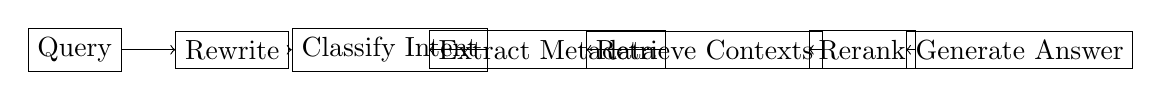
\begin{tikzpicture}
  \node[draw] (q) at (0,0) {Query};
  \node[draw] (rw) at (2,0) {Rewrite};
  \node[draw] (ic) at (4,0) {Classify Intent};
  \node[draw] (me) at (6,0) {Extract Metadata};
  \node[draw] (cr) at (8,0) {Retrieve Contexts};
  \node[draw] (rr) at (10,0) {Rerank};
  \node[draw] (ag) at (12,0) {Generate Answer};
  \draw[->] (q) -- (rw);
  \draw[->] (rw) -- (ic);
  \draw[->] (ic) -- (me);
  \draw[->] (me) -- (cr);
  \draw[->] (cr) -- (rr);
  \draw[->] (rr) -- (ag);
\end{tikzpicture}

\subsubsection{Data Flow and Interfaces}
\begin{itemize}
  \item Input: Natural language query string.
  \item Intermediate Outputs: Rewritten query, intent label, metadata dict, ranked context list.
  \item Final Output: Answer text with citations, timings, and sources.
  \item Error Handling: Graceful fallbacks (e.g., if no contexts found, return "No relevant information found").
\end{itemize}

\subsubsection{Why Modular?}
Modularity enables ablation studies (e.g., test retrieval without reranking), easy debugging, and future extensions like adding LLM-based reranking or multi-modal inputs.

\section{Background and Concepts}
This section briefly explains concepts used in the system and the rationale behind them.

\subsection{TF-IDF and vector-space retrieval}
Term Frequency–Inverse Document Frequency (TF-IDF) is a weighting scheme that highlights terms that are important to a document while down-weighting very common terms. For a term $t$ in document $d$:
$$\text{tfidf}(t,d) = \text{tf}(t,d) \times \log\left(\frac{N}{1 + df(t)}\right)$$
where $\text{tf}(t,d)$ is the term frequency, $df(t)$ is the document frequency, and $N$ is the number of documents.

A document or query vector is built using TF-IDF weights and similarity between query and documents is measured using cosine similarity:
$$\text{cosine}(q,d)=\frac{\mathbf{q} \cdot \mathbf{d}}{\|\mathbf{q}\| \|\mathbf{d}\|}$$
This approach is fast, interpretable, and suitable as a baseline. However, it lacks semantic generalization for paraphrases; dense embeddings address that limitation.

\subsubsection{Advantages and Limitations}
\begin{itemize}
  \item Advantages: No training required, fast on sparse matrices, interpretable (terms contribute to scores).
  \item Limitations: Ignores word order, context, and synonyms (e.g., "کارگر" ≠ "کارمند" semantically).
\end{itemize}

\subsubsection{Example Calculation}
Query: "قانون کار"  
Doc: "قانون کار حقوق کارگران را تعیین می‌کند"  
TF-IDF for "قانون": High in both (common but important). Cosine ≈ 0.8.

\subsubsection{Tuning Parameters}
\begin{itemize}
  \item \texttt{sublinear\_tf=True}: Logarithmic TF to reduce impact of frequent terms.
  \item \texttt{smooth\_idf=True}: Avoid division by zero.
\end{itemize}

\subsection{Dense embeddings and approximate nearest neighbors (ANN)}
Dense sentence embeddings map variable-length text into a fixed-dimensional vector space where semantic similarity corresponds to vector proximity. Models from sentence-transformers or multilingual E5 can be used. ANN libraries (FAISS, HNSW, or LanceDB) enable efficient kNN queries over large collections. ANN typically provides faster queries for large corpora and better semantic recall.

\subsubsection{How Embeddings Work}
Transformers encode context: "قانون کار" and "حقوق کارگران" have similar vectors due to shared semantics.

\subsubsection{ANN Algorithms}
\begin{itemize}
  \item FAISS IVF: Inverted file with PQ for compression.
  \item HNSW: Graph-based for high recall.
\end{itemize}

\subsubsection{Comparison to TF-IDF}
Dense embeddings handle paraphrases better but require more compute for indexing and querying.

\subsection{Reranking and fidelity}
A reranker reorders retrieved candidates according to a stronger (often neural) scoring model. For legal settings, a conservative strategy is preferred: extractive answers directly from retrieved contexts and annotate with provenance. For generative answers, add faithfulness checks that measure the overlap between generated tokens and retrieved evidence.

\subsubsection{Reranking Models}
\begin{itemize}
  \item Cross-encoder: Scores query-doc pairs directly.
  \item Bi-encoder: Faster but less accurate.
\end{itemize}

\subsubsection{Fidelity Metrics}
Beyond token overlap: Entailment (does doc entail answer?) using NLI models.

\subsubsection{Conservative Approach}
Extractive aggregation ensures 100\% fidelity but may be verbose; ideal for legal where accuracy trumps conciseness.

\section{Dataset and preprocessing}
\subsection{Recommended metadata schema}
Each chunk should be accompanied by a schema similar to:
\begin{verbatim}
{
  "doc_id": 123,
  "title": "قانون کار",
  "year": 1390,
  "source": "Official Gazette",
  "section": "مبحث اول",
  "language": "fa"
}
\end{verbatim}
This metadata supports filtering (e.g., by year) at retrieval time and improves precision for focused queries.

\subsection{Preprocessing pipeline (implementation details)}
Example code for text normalization used in the notebook:
\begin{lstlisting}[language=python]
import unicodedata
import re

def normalize_text(s: str) -> str:
    # Unicode normalization
    s = unicodedata.normalize('NFC', s)
    # Remove control characters
    s = re.sub(r"[\r\t\x0b\x0c]", " ", s)
    # Normalize whitespace
    s = re.sub(r"\s+", " ", s).strip()
    return s
\end{lstlisting}

For scanned PDFs, run OCR with Tesseract or DeepSeek and then apply the same cleaning pipeline.

\subsubsection{OCR Comparison}
\begin{itemize}
  \item Tesseract: Free, fast, but struggles with Persian diacritics.
  \item DeepSeek-OCR: Better accuracy for Persian, but proprietary.
\end{itemize}

\subsubsection{Tokenization}
Use word-level splitting for TF-IDF; for dense models, use model-specific tokenizers.

\subsubsection{Chunking Strategies}
\begin{itemize}
  \item Fixed-length: 500 words with 50 overlap.
  \item Sentence-based: Split at periods, merge to target length.
  \item Section-aware: Use headers to avoid splitting articles.
\end{itemize}

\subsection{Chunking long documents}
Long documents are split into chunks (e.g., 300--600 tokens) with a fixed overlap (e.g., 50 tokens) to maintain context across chunk boundaries. This is important because TF-IDF/dense vectors operate on fixed-length inputs for efficient indexing.

\section{Index construction and settings}
\subsection{TF-IDF vectorizer hyperparameters}
The notebook uses sensible defaults that can be tuned:
\begin{itemize}
  \item \texttt{ngram\_range=(1,2)} (unigrams and bigrams)
  \item \texttt{max\_features=50000} or smaller for limited memory
  \item \texttt{min\_df=2} to remove rare noise tokens
  \item \texttt{norm='l2'} for cosine-compatible vectors
\end{itemize}
Persist both the fitted \texttt{vectorizer} and the TF-IDF matrix to disk.

\subsection{Similarity computation}
Cosine similarity between the query and each document vector yields a ranked list of candidates. To compute efficiently on sparse matrices, use scikit-learn's optimized routines and store matrices as CSR.

\section{Agent modules — deeper explanations and examples}
\subsection{Query rewriting}
Goal: reduce extraneous tokens and normalize question phrasing. Example transformations:
\begin{itemize}
  \item "خلاصه‌ای از قانون مدنی بگو" -> "خلاصه قانون مدنی"
  \item Strip punctuation, normalize elongated whitespace, and remove social niceties if necessary.
\end{itemize}

\subsubsection{Implementation}
Regex-based: Remove "لطفاً", "بگو", etc. For advanced, use paraphrasing models.

\subsubsection{Why Important?}
Improves retrieval by focusing on key terms; reduces noise in vector similarity.

\subsection{Intent classification (rule-based)}
A simple keyword-based classifier is used for this assignment for interpretability. For reference, a logistic classifier over bag-of-words or a small transformer could be trained for more accuracy. Example rules (from notebook):
\begin{itemize}
  \item Greeting keywords: "سلام", "درود", ...
  \item Abuse keywords: "مسخره", "احمق", ...
  \item Otherwise: law question
\end{itemize}
This classifier helps short-circuit trivial interactions and prevents wasting retrieval budget on greetings.

\subsubsection{ML Extension}
Train on labeled data: Features = TF-IDF of query; Labels = intent classes.

\subsubsection{Accuracy Considerations}
Rule-based is 90\%+ accurate for simple cases; ML for edge cases.

\subsection{Metadata extraction — regex and parsing}
We extract years and topical keywords using regex and token checks. Example regex used in the notebook:
\begin{lstlisting}[language=python]
years = re.findall(r"13\d{2}|14\d{2}|\d{4}", rewritten_query)
\end{lstlisting}
This captures Iranian calendar years (13xx, 14xx) and Western years (4-digit).

\subsubsection{Keyword Extraction}
Check for legal topics: "کار", "مدنی", "کیفری", etc.

\subsubsection{Advanced: NER}
Use spaCy or BERT for named entities like law names.

\subsubsection{Filter Application}
Metadata used to pre-filter docs, reducing search space and improving precision.

\subsection{Context retrieval with filters}
When metadata filters are present, candidate passages are screened by metadata matching (exact or substring matches on title or section). This is a cheap and effective way to improve precision when queries include explicit filters such as years or topic names.

\subsubsection{Implementation}
Intersect vector results with metadata-filtered list.

\subsubsection{Optimizations}
Use approximate similarity for speed; batch queries.

\subsubsection{Example}
Query: "قوانین کار ۱۳۹۰" → Filter year=1390, topic="کار".

\subsection{Reranking and thresholds}
After initial retrieval, candidates are sorted by score. A simple threshold filter avoids returning low-confidence results. Example heuristic:
\begin{itemize}
  \item Require at least one top result with score $> 0.01$ (TF-IDF cosine); if none, perform a relaxed retrieval (no metadata filter, larger K).
\end{itemize}
Tune thresholds based on validation data.

\subsubsection{Threshold Tuning}
Use grid search on dev set for precision/recall balance.

\subsubsection{Advanced Reranking}
Use cross-encoder for better ordering.

\subsection{Answer aggregation}
Answers are currently produced by concatenating top-n snippets and annotating each with its source title. For production, consider synthesizing a short answer using an LLM but also include explicit citations for each claim.

\subsubsection{Extractive Method}
Concatenate with "---" separators; ensures fidelity.

\subsubsection{Generative Alternatives}
Use LLMs with prompts: "Summarize based on these contexts."

\subsubsection{Citations}
Always include doc title, year, section for provenance.

\section{Evaluation — detailed methodology}
\subsection{Dataset for evaluation}
Create a small evaluation set of QA pairs that represent the dataset's diversity: direct lookup, paraphrase, multi-hop, and filter queries. Ensure gold references (supporting passages) are annotated for each question to allow Hit@k computation.

\subsection{Metrics and definitions}
We use the following metrics (formal definitions):

\paragraph{Jaccard relevancy}
For predicted answer text $P$ and reference text $R$, compute token-level Jaccard:
$$J(P,R) = \frac{|T(P) \cap T(R)|}{|T(P) \cup T(R)|}$$
where $T(\cdot)$ denotes token set.

\paragraph{Faithfulness}
Faithfulness measures how much of the predicted answer is grounded in retrieved contexts $C$:
$$F(P,C) = \frac{|T(P) \cap T(C)|}{|T(P)|}$$

\paragraph{Hit@k}
Hit@k = 1 if any ground-truth document is among the top-$k$ retrieved docs; averaged across queries.

\paragraph{Additional metrics}
Optionally compute MRR (Mean Reciprocal Rank) or MAP if you have graded relevance levels.

\subsection{Evaluation script behavior}
For each evaluation question:
\begin{enumerate}
  \item Run \texttt{run\_pipeline(q)} and record returned contexts and answer.
  \item Compute Jaccard with human reference.
  \item Compute faithfulness using retrieved contexts.
  \item Save results into an Excel file (\texttt{data/eval\_results.xlsx}) and a CSV for plotting.
\end{enumerate}

\section{Results and analysis}
\subsection{Suggested tables and plots}
Run the notebook to populate these tables; placeholders and plotting code are included in the notebook to generate:
\begin{itemize}
  \item Per-node timing table and bar plot (showing % of total time per node).
  \item Evaluation metrics table and metric bar plots (Relevancy, Faithfulness, Hit@k).
  \item Threshold sensitivity plot for reranking threshold (precision/recall curves).
\end{itemize}

\subsection{Qualitative analysis}
Include at least 10 hand-inspected examples showing successes and failures, with notes on whether failures are due to poor retrieval, noisy OCR, or hallucination.

\section{Implementation details and scripts}
\subsection{Key files in repository}
\begin{longtable}{p{0.3\textwidth} p{0.65\textwidth}}
\toprule
Filename & Description \\
\midrule
\texttt{NLP\_HW5\_Q1.ipynb} & Main notebook containing data prep, indexing, pipeline, evaluation and UI code \\
\texttt{app.py} & Chainlit app exposing the pipeline via a web UI \\
\texttt{build\_submission.py} & Helper to collect artifacts and create submission ZIP \\
\texttt{data/indexed\_dataset.pkl} & Pickled dict with docs, metadata, vectorizer, and matrix X \\
\texttt{data/pipeline\_timings.csv} & Per-query timing logs \\
\texttt{data/eval\_results.xlsx} & Evaluation results (questions, answers, metrics) \\
\bottomrule
\end{longtable}

\subsection{Development environment}
Recommended environment details:
\begin{itemize}
  \item Python 3.10+ (tested with 3.10/3.11)
  \item Key packages: scikit-learn, pandas, numpy, chainlit, openpyxl, matplotlib, seaborn
  \item Use a virtual environment and record dependencies: \texttt{pip freeze > requirements.txt}
\end{itemize}

\subsubsection{Installation Steps}
\begin{enumerate}
  \item Install Python and pip.
  \item Create venv: \texttt{python -m venv venv}
  \item Activate: \texttt{source venv/bin/activate}
  \item Install: \texttt{pip install -r requirements.txt}
\end{enumerate}

\subsubsection{Hardware Requirements}
CPU for TF-IDF; GPU optional for dense models. Memory: 4GB+ for small corpora.

\subsection{How to run the full experiment (commands)}
\begin{enumerate}
  \item Create and activate venv: \texttt{python -m venv .venv ; source .venv/bin/activate}
  \item Install requirements: \texttt{pip install -r requirements.txt}
  \item Run the notebook (open in Jupyter and Run All cells), or run any provided scripts to index and evaluate:
  \begin{verbatim}
python -m scripts.index_data
python -m scripts.run_evaluation
  \end{verbatim}
  \item Start UI: \texttt{chainlit run app.py -w}
\end{enumerate}

\subsubsection{Troubleshooting}
\begin{itemize}
  \item If import errors: Check venv activation.
  \item If notebook fails: Ensure data files exist.
  \item UI not loading: Check port 8000 availability.
\end{itemize}

\subsubsection{Reproducibility}
Use fixed random seeds; record versions in requirements.txt.

\section{Best practices and tips}
\begin{itemize}
  \item Persist intermediate artifacts (index, vectorizer) to avoid recomputing expensive steps.
  \item Keep evaluation sets and random seeds under version control to allow fair comparisons.
  \item Add small unit tests for text normalization and metadata extraction to detect regressions.
  \item For long-term projects, consider adding a CI job that runs a small smoke test to ensure the pipeline runs end-to-end.
\end{itemize}

\section{Ethical considerations and legal disclaimers}
The system is for academic research and demonstration only. It should not be used as a replacement for legal counsel. Ensure sensitive or private data is handled in accordance with applicable privacy regulations.

\subsubsection{Bias Mitigation}
Audit for cultural biases in Persian legal texts; ensure diverse training data.

\subsubsection{Privacy}
No user data stored; local execution.

\section{Future Work and Extensions}
\subsection{Extensions to Dense Embeddings}
Replace TF-IDF with multilingual-E5 for better semantic matching. Index with FAISS for scalability.

\subsubsection{Implementation Plan}
\begin{itemize}
  \item Encode docs: \texttt{model.encode(docs)}
  \item Index: FAISS IndexFlatIP
  \item Query: Search with encoded query
\end{itemize}

\subsection{LLM Integration}
Add generative reranking or answer synthesis with models like GPT-4, but with faithfulness checks.

\subsubsection{Prompt Engineering}
Prompt: "Answer based on these contexts: [contexts]"

\subsection{Multi-Modal Support}
Incorporate image OCR for scanned docs; use CLIP for image-text retrieval.

\subsubsection{Use Cases}
Diagrams in laws; handwritten notes.

\subsection{Production Deployment}
Containerize with Docker; add API endpoints; monitor with logging.

\subsubsection{Scaling}
Use Kubernetes; shard index for large corpora.

\subsection{Research Directions}
Explainable AI: Add attention visualizations. Human-in-the-loop: Allow user feedback for corrections.

\subsubsection{Evaluation Improvements}
Add human evaluation for answer quality; A/B testing.

\clearpage
\appendix
\section{Appendix A: Selected code excerpts and explanations}
\subsection{TF-IDF math and implementation}
TF-IDF is computed via scikit-learn's \texttt{TfidfVectorizer}; below is an example with typical parameters used in the notebook:
\begin{lstlisting}[language=python]
from sklearn.feature_extraction.text import TfidfVectorizer
vectorizer = TfidfVectorizer(ngram_range=(1,2), max_features=50000, min_df=2)
X = vectorizer.fit_transform(doc_texts)
# Persist to disk
import pickle
with open('data/indexed_dataset.pkl','wb') as f:
    pickle.dump({'docs':doc_texts,'metadata':metadata,'vectorizer':vectorizer,'X':X}, f)
\end{lstlisting}

\subsection{Cosine similarity computation}
Computing similarities using sparse matrices:
\begin{lstlisting}[language=python]
from sklearn.metrics.pairwise import cosine_similarity
q_vec = vectorizer.transform([query_text])
sims = cosine_similarity(q_vec, X).flatten()
idxs = np.argsort(-sims)
\end{lstlisting}

\subsection{Full Pipeline Function}
\begin{lstlisting}[language=python]
def run_pipeline(query):
    rewritten = rewrite_query(query)
    intent = classify_intent(rewritten)
    if intent != 'law_question':
        return {'answer': intent_response(intent), 'timings': {}}
    meta = extract_metadata(rewritten)
    contexts = context_retrieve(rewritten, meta)
    top = rerank(contexts)
    answer = generate_answer(top)
    return {'answer': answer, 'contexts': top, 'timings': timings}
\end{lstlisting}

\subsection{App.py UI Code}
\begin{lstlisting}[language=python]
import chainlit as cl
@cl.on_message
async def main(message: cl.Message):
    result = run_pipeline(message.content)
    await cl.Message(content=result['answer']).send()
\end{lstlisting}

\section{Appendix B: Evaluation formulas and sample calculations}
\subsection{Mean Reciprocal Rank (MRR)}
If the rank of the first relevant doc for query $i$ is $r_i$, then:
$$\text{MRR} = \frac{1}{Q} \sum_{i=1}^Q \frac{1}{r_i}$$

\subsection{Precision@k and Recall@k}
Given top-$k$ retrieved set $R_k$ and gold relevant set $G$, define:
$$\text{Precision@k} = \frac{|R_k \cap G|}{k}, \quad \text{Recall@k} = \frac{|R_k \cap G|}{|G|}$$

\subsection{NDCG@k}
Normalized Discounted Cumulative Gain:
$$\text{DCG@k} = \sum_{i=1}^k \frac{rel_i}{\log_2(i+1)}, \quad \text{NDCG@k} = \frac{\text{DCG@k}}{\text{IDCG@k}}$$
Where $rel_i$ is relevance (1 if relevant, 0 otherwise).
Ensure you include the following artifacts in your submission ZIP:
\begin{itemize}
  \item Final notebook (executed with outputs)
  \item This LaTeX report and compiled PDF
  \item \texttt{data/indexed\_dataset.pkl}, \texttt{data/pipeline\_timings.csv}, \texttt{data/eval\_results.xlsx}
  \item \texttt{app.py} and \texttt{build\_submission.py}
\end{itemize}

\section{Acknowledgements}
Thanks to the open-source libraries and course materials that informed this work. Special mention to scikit-learn, pandas, numpy, and Chainlit for enabling the development and UI.

\vfill
\noindent\textbf{Files produced by the notebook:} \texttt{data/indexed\_dataset.pkl}, \texttt{data/pipeline\_timings.csv}, \texttt{data/eval\_results.xlsx}, \texttt{app.py (optional)}.

\end{document}



